\documentclass[12pt]{article}
\usepackage{graphicx}
\usepackage{cite}
\graphicspath{ {../diagram/} }
\title{Neural Network Compression}
\author{David Turner}

\begin{document}

\begin{titlepage}
\maketitle
\end{titlepage}

\section{Abstract}

\section{Introduction}
Motivations and goals. There should also be the main hypothesis of the project. Why is this an interesting hypothesis to investigate. Use illistrations

\section{Literature Review}
15-20 pages
\subsection{Processor Architectures for deep learning}

\subsection{High Performance Devices}
Include numbers here relating to memory and performance metrics from papers including speed, accuracy, model size
\subsubsection{GPUs}
\subsubsection{TPUs}
\subsubsection{CPUs}

\subsection{Low Power Edge Devices}
Numbers of memory and performance metrics for each of these
\subsubsection{FPGAs}
\begin{itemize}
\item
General Structure
\item
What makes them a good choice?
\end{itemize}

\subsubsection{USB Accelerators}
\begin{itemize}
\item
Intel Neural Compute Stick 
\begin{itemize}
\item
VPU Structure
\item
vpu figures
\end{itemize}
\item
Google Coral USB Acellerator
\begin{itemize}
\item
TPU At Edge

\end{itemize}
	

\end{itemize}

\subsubsection{Embedded GPUs}
Embedded within phones for example arm stuff and apple
\subsubsection{Smart Home}
Google home now has neural processing units
\subsubsection{Edge Custom Solutions}
\begin{itemize}
\item
Nvidia Jetson Line
\item
NVIDIA EGX
\item
Graphcore
\item
Qualcomm
\item
adapteva
\item
viatech
\item
mediatek - Supplimenting cloud ai chip in device NeuroPilot
\item
Kalray
\item
AWS Inferentia
\item
Arm
\item
Intel® Nervana™ Neural Network processors
\item 
custom asic
\end{itemize}

\section{Compression Techniques}
\subsection{Methods/Algorithms}
\subsubsection{Pruning}
\subsubsection{Quantization}
\subsubsection{Knowledge Distillation}
\subsubsection{Regularization}
\subsubsection{Conditional Computation}

\subsection{Frameworks}
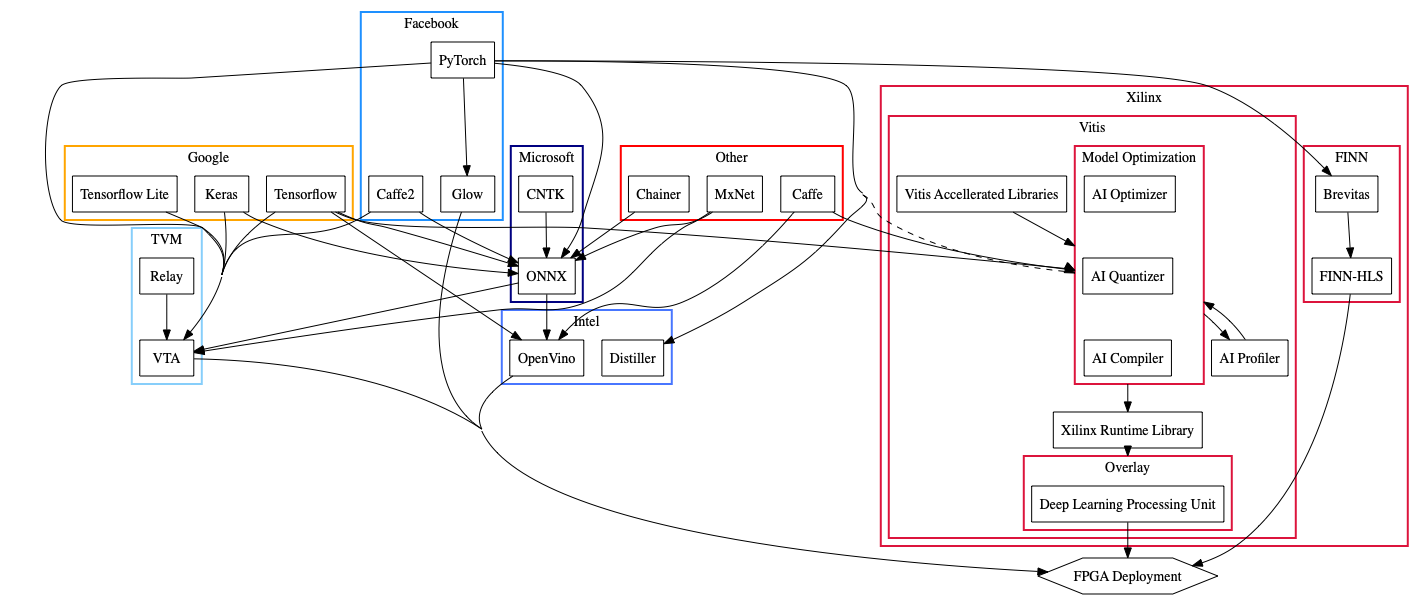
\includegraphics[width=\textwidth]{diagram.png}
\subsubsection{Intel Distiller}
\subsubsection{FINN}
\subsubsection{Intel OpenVino}
\subsubsection{Xilinx Vitis}

\section{Requirements Analysis}
3 pages atleast \cite{RN54}

\subsection{Research Questions}
\subsection{hypothesis}
\subsection{Aim}
\subsection{Objectives}

\section{Methodology}
Datasets
Preliminary ideas fo model or system
Experimantal setup and evaluation

\section{Project Plan}
How will each objective achieve the aim to allow for the hypothesis to be proved or disproved

\subsection{Gantt Chart}

\subsection{Risk Analysis}

\newpage
\bibliography{bibliography}
\bibliographystyle{plain}


\end{document}

